%\chapterimage{Geometrijska.jpg} % Chapter heading image

\chapter{Geometrijska optika}
V tem poglavju bomo na kratko predstavili geometrijsko optiko,
v kateri svetlobo obravnavamo kot ravne žarke. Zapisali bomo
žarkovno enačbo, vpeljali matrike ABCD za račun prehoda svetlobe
skozi optične elemente in na
primerih pokazali njihovo uporabo. Na koncu bomo opisali 
delovanje nekaterih preprostih optičnih naprav. 

\section{Fermatov teorem in optična pot}
V uvodnem zgodovinskem pregledu smo zapisali Fermatov teorem, 
ki pravi, da svetloba med dvema točkama potuje po tisti poti, 
za katero potrebuje najmanj časa. Označimo
hitrost svetlobe v snovi s $c$ in na splošno se  $c$ razlikuje
od hitrosti svetlobe v praznem prostoru $c_0$. Razmerje med
hitrostjo svetlobe v praznem prostoru in njeno hitrostjo
v snovi opisuje lomni količnik $n$. Velja:
\boxeq{eq:c}{
c = \frac{c_0}{n}.
}
Hitrost svetlobe v praznem prostoru je
po definiciji enaka $c_0 = 299\,\,792\,\,458~\si{m/s}$, 
lomni količnik pa je odvisen od snovi in frekvence svetlobe: za vidno svetlobo
je v vodi približno $1,3$, v steklih okoli $1,4$--$1,9$ in v diamantu $2,4$.

Naj svetloba potuje po snovi z lomnim količnikom $n$. Celotno pot, ki 
jo svetloba opravi od začetne do končne točke, razdelimo na kratke intervale 
poti $ds$. Za del poti $ds$ potrebuje svetloba čas $dt$, ki ga zapišemo kot:
\begin{equation}
 dt = \frac{ds}{c} = \frac{ds}{c_0/n} = \frac{nds}{c_0}.
\label{eq:02_02}
\end{equation}
Fermatov teorem pravi, da svetloba potuje po poti, za katero velja:
\beq
\int_1^2 dt = \int_1^2 \frac{nds}{c_0} = \mathrm{min}.
\label{eq:02_03}
\eeq
Če je lomni količnik konstanten, svetloba potuje naravnost in 
ne spreminja smeri. Na splošno pa se lomni količnik spreminja s 
krajem, zato teorem prepišemo v:
\boxeq{eq:02_04}{
S = \int_1^2 n(\mathbf{r})ds = \mathrm{min}.
}
Celotni integral $S$ imenujemo optična pot, ki se od geometrijske poti razlikuje v tem,
da upošteva tudi lomni količnik snovi. 
Zapisani izraz imenujemo princip najmanjše optične poti oziroma najmanjše optične akcije. 
Problem je podoben principu najmanjše akcije v klasični mehaniki, zato včasih govorimo  
tudi o Langrangeevi oziroma Hamiltonovi optiki.
\begin{remark}
Princip najkrajše optične poti lahko formalno izpeljemo z 
obravnavo valovnih front in žarkov v valovni optiki, če naredimo limito $\lambda \to 0$.
Tako lahko izhajajoč iz Maxwellovih enačb pokažemo pravilnost Fermatovega teorema.
\end{remark}

\begin{example}
{\bf Izpeljava lomnega zakona iz Fermatovega teorema.}
Naj svetlobni žarek vpada na ravno mejo dveh snovi. Levo od meje je snov 
z lomnim količnikom $n_1$, desno pa snov z lomnim količnikom $n_2$. Naj svetloba
potuje od točke 1, ki jo izberemo na oddaljenosti $z_1$ levo 
od meje, do točke 2 na oddaljenosti $z_2$ desno od meje. Vzdolžna razdalja med obema
točkama naj bo $x$ (slika~\ref{fig:02_FerLom}). 
\begin{figure}[ht]
\centering
\def\svgwidth{100truemm} 
\input{slike/02_FerLom.pdf_tex}
\caption{K izračunu loma na meji dveh snovi}
\label{fig:02_FerLom}
\end{figure}

Naša naloga je poiskati pot žarka svetlobe od točke 1 do točke 2 ob pogoju, 
da je skupna optična pot najkrajša.
Celotno optično pot zapišemo kot:
\begin{equation}
S = n_1 s_1 + n_2 s_2 = n_1 \sqrt{x_1^2+z_1^2}\, +\, n_2 \sqrt{x_2^2+z_2^2}.
\label{eq:02_05}
\end{equation}
Izrazimo parameter $x_2$ z lego iskane točke $x_1$: 
\begin{equation}
S = n_1 \sqrt{x_1^2+z_1^2}\, +\, n_2 \sqrt{(x-x_1)^2+z_2^2}.
\label{eq:02_06}
\end{equation}
Najkrajšo optično pot izračunamo tako, da poiščemo vrednost $x_1$, 
pri kateri je odvod optične poti po $x_1$ enak nič. Zapišemo:
\begin{equation}
\frac{dS}{dx_1} = \frac{2 n_1 x_1}{2 \sqrt{x_1^2+z_1^2}}+
\frac{-2n_2 (x-x_1)}{2 \sqrt{(x-x_1)^2+z_2^2}} = 0.
\label{eq:02_07}
\end{equation}
Vpeljemo vpadni kot $\alpha$ glede na normalo na mejo snovi (slika~\ref{fig:02_FerLom}):
\begin{equation}
\sin \alpha = \frac{x_1}{\sqrt{x_1^2+z_1^2}}.
\label{eq:02_08}
\end{equation}
Lomni kot $\beta$ naj bo kot med smerjo žarka v drugi snovi in normalo na mejo snovi: 
\begin{equation}
\sin \beta = \frac{x_2}{\sqrt{x_2^2+z_2^2}} = \frac{(x-x_1)}{\sqrt{(x-x_1)^2+z_2^2}}.
\label{eq:02_09}
\end{equation}
Vstavimo enačbi~(\ref{eq:02_08}) in (\ref{eq:02_09}) v enačbo~(\ref{eq:02_07})
in dobimo lomni zakon v znani obliki:
\boxeq{eq:lomnizakon}{
n_1 \sin \alpha = n_2 \sin \beta.
}
Na podoben način izpeljemo tudi odbojni zakon, tako da izračunamo 
najkrajšo optično pot med točkama 1 in 3. Dobimo:
\boxeq{eq:odbojnizakon}{
\tilde{\alpha} = \alpha.
}
\end{example}

\section{Žarkovna enačba}
Poglejmo, kako izračunamo najkrajšo optično pot v primeru, ko 
meja med dvema snovema ni ostra, ampak se lomni količnik zvezno spreminja. 
Naj bo lomni količnik v splošnem funkcija kraja: $n = n(\mathbf{r}) = n(x,y,z)$.
Numerično se naloge lotimo tako, da snov razdelimo
na kratke odseke in na mejah med njimi uporabimo lomni ali odbojni zakon.
Analitično problem rešujemo z uporabo Euler-Lagrangeeve enačbe za minimum
funkcionala optične poti $S$:
\begin{equation}
 S = \int_1^2 n(x,y,z) ds  = \int_1^2 n(x,y,z)\,|\mathbf{v}|\,dt  = 
 \int_1^2 n(x,y,z) \sqrt{\dot{x}^2+ \dot{y}^2+\dot{z}^2} dt,
 \label{eq:02_10}
\end{equation}
pri čemer pika označuje odvod posamezne koordinate po času. Integrand
enačbe predstavlja Langrangian $L$, ki je funkcija treh koordinat in njihovih
odvodov.
\begin{equation}
L(x, y, z, \dot{x}, \dot{y}, \dot{z}) = n(x,y,z) \sqrt{\dot{x}^2+ \dot{y}^2+\dot{z}^2}.
\label{eq:02_11}
\end{equation}
Lagrangian vstavimo v Euler-Lagrangeevo enačbo\footnote{~Glej npr. P. Prelovšek, {\it Klasična
mehanika}, skripta, 2013.} in za koordinato $x$ dobimo:
\begin{equation}
 \frac{d}{dt}\left(\frac{\partial L}{\partial \dot{x}}\right) - 
 \frac{\partial L}{\partial x} = 0.
 \label{eq:02_12}
\end{equation}
Vstavimo Langrangian (enačba~\ref{eq:02_11}) 
v enačbo~(\ref{eq:02_12}) in dobimo:
\begin{equation}
\frac{d}{dt}\left(n \frac{\dot{x}}{\sqrt{\dot{x}^2+ \dot{y}^2+\dot{z}^2}} \right)
 = \frac{\partial n}{\partial x}\sqrt{\dot{x}^2+ \dot{y}^2+\dot{z}^2}.
  \label{eq:02_13}
\end{equation}
Pomnožimo enačbo z $dt/ds$:
\begin{equation}
\frac{d}{dt}\left(n \frac{\dot{x}}{\sqrt{\dot{x}^2+ \dot{y}^2+\dot{z}^2}} \right)
\frac{dt}{ds}
 = \frac{\partial n}{\partial x}\frac{\sqrt{\dot{x}^2+ \dot{y}^2+\dot{z}^2}\,dt}{ds}.
  \label{eq:02_14}
\end{equation}
Na desni strani enačbe uporabimo zvezo:
\begin{equation}
 \sqrt{\dot{x}^2+ \dot{y}^2+\dot{z}^2} dt = ds,
 \label{eq:02_15}
\end{equation}
na levi strani pa verižno pravilo odvajanja, po katerem lahko pokrajšamo $dt$. Dobimo:
\begin{equation}
 \frac{d}{ds} \left( n \frac{dx}{dt\sqrt{\dot{x}^2+ \dot{y}^2+\dot{z}^2}} \right)=
 \frac{\partial n}{\partial x}.
 \label{eq:02_16}
\end{equation}
Enačbo~(\ref{eq:02_15}) uporabimo še enkrat v oklepaju na levi strani. Sledi:
\begin{equation}
 \frac{d}{ds} \left( n\, \frac{dx}{ds} \right)=
 \frac{\partial n}{\partial x}.
  \label{eq:02_17}
\end{equation}
Podobni enačbi zapišemo še za koordinati $y$ in $z$, nato vse tri enačbe
združimo v enotno žarkovno enačbo:
\boxeq{eq:zarkovnaenacba}{
\nabla n = \frac{d}{ds} \left( n \frac{d\mathbf{r}}{ds}\right)\!.
}
Rešitev žarkovne enačbe poda trajektorijo optičnega žarka v parametrični 
obliki $\mathbf{r}(s)$. Z uporabo zveze $ds = dz (1+(dx/dz)^2+(dy/dz)^2)^{1/2}$
lahko enačbo prevedemo na sistem diferencialnih enačb za $x(z)$ in $y(z)$. Reševanje
tega sistema enačb je na splošno zelo zapleteno.

\begin{example}
{\bf Žarkovna enačba v homogeni snovi.} Naj svetloba potuje po snovi,
v kateri je lomni količnik konstanten. Potem je $\nabla n = 0$ in 
\begin{equation}
0 = \frac{d}{ds}\left( n \frac{d\mathbf{r}}{ds} \right) = 
n \frac{d^2 \mathbf{r}}{ds^2}.
 \label{eq:02_18}
\end{equation}
Rešitev te enačbe je ravni žarek:
\begin{equation}
 \mathbf{r} = \mathbf{a}_0+\mathbf{a}_1\,s,
  \label{eq:02_19}
\end{equation}
pri čemer vektor $\mathbf{a}_0$ opisuje lego začetne točke, 
vektor $\mathbf{a}_1$ pa ima smer od začetne do končne točke.
\end{example}

\subsection*{Obosni približek žarkovne enačbe}
V optiki pogosto privzamemo, da smer širjenja svetlobe le malo 
odstopa od neke dane smeri. Naj bo to smer $z$, ki jo imenujemo
optična os sistema. Zaradi enostavnosti se omejimo na ravninski primer, 
tako da trajektorijo žarka opazujemo v ravnini $xz$ 
(slika~\ref{fig:02_FerOs}). Lomni količnik naj bo funkcija $n= n(x)$.
\begin{figure}[ht]
\centering
\def\svgwidth{90truemm} 
\input{slike/02_FerOs.pdf_tex}
\caption{K zapisu žarkovne enačbe v obosnem približku}
\label{fig:02_FerOs}
\end{figure}

Predpostavko, da se žarek širi pretežno v smeri $z$ in od te smeri 
le malo odstopa, matematično zapišemo s pogojem:
\begin{equation}
 \frac{dx}{dz}\ll 1.
  \label{eq:02_20}
\end{equation}
Iz tega sledi, da za naklon žarka $\vartheta$, ki ga na danem mestu izračunamo kot:
\begin{equation}
\vartheta = \frac{dx}{dz}
 \label{eq:02_21}
\end{equation}
velja $\sin \vartheta \approx \tan \vartheta \approx \vartheta \ll 1$.
Upoštevajoč enačbo~(\ref{eq:02_20}) zapišemo:
\begin{equation}
ds = \sqrt{dx^2+dz^2} = \sqrt{1+\left(\frac{dx}{dz}\right)^2}\,\,dz \approx dz.
\label{eq:02_22}
\end{equation}
Predpostavki, da se žarek širi približno vzdolž osi $z$, pravimo
obosni ali paraksialni približek. V nadaljevanju se ga bomo še velikokrat 
posluževali. Žarkovno enačbo (enačba~\ref{eq:zarkovnaenacba}) v obosnem približku
zapišemo kot:
\begin{equation}
 \frac{dn}{dx} = \frac{d}{dz}\left(n(x)\,\frac{dx}{dz}\right) = n(x)\,\frac{d^2x}{dz^2}
  \label{eq:02_23}
\end{equation}
oziroma
\boxeq{eq:02_24}{
\frac{d^2x}{dz^2} = \frac{1}{n(x)} \frac{dn}{dx}.
}

\begin{example}
{\bf Žarkovna enačba v snovi s paraboličnim profilom
lomnega količnika.} Izračunajmo trajektorijo žarka svetlobe v 
obosnem približku v snovi, v kateri se lomni količnik parabolično 
spreminja z oddaljenostjo od osi $z$.  Odvisnost lomnega količnika 
od oddaljenosti $x$ od osi $z$ zapišemo kot:
\begin{equation}
 n(x) = n_0 \left(1-\frac{\alpha^2\,x^2}{2}\right)\!,
 \label{eq:02_25}
\end{equation}
pri čemer je $\alpha x$ majhen.
Vstavimo izraz za lomni količnik (enačba~\ref{eq:02_25}) v obosni približek
žarkovne enačbe (enačba~\ref{eq:02_24}) in dobimo:
\begin{equation}
 \frac{d^2x}{dz^2}= \frac{1}{n(x)}\frac{dn}{dx} = 
 \frac{-n_0 \alpha^2x}{n_0 \left(1-\alpha^2\,x^2/2\right)} 
 \approx -\frac{n_0\alpha^2x}{n_0} = -\alpha^2x.
 \label{eq:02_26}
\end{equation}
Enačbo~(\ref{eq:02_26}) preprosto rešimo in dobimo splošno 
obliko trajektorije:
\begin{equation}
 x(z) = A \cos (\alpha z) + B \sin (\alpha z).
  \label{eq:02_27}
\end{equation}
Naj bo v izhodišču pri $z=0$ žarek na oddaljenosti $x_0$ 
in naj se širi pod kotom $\vartheta_0$. 
Z upoštevanjem začetnih pogojev dobimo rešitev:
\begin{equation}
x (z) = x_0 \cos(\alpha z) + \frac{\vartheta_0}{\alpha} \sin (\alpha z).
 \label{eq:02_28}
\end{equation}
Rešitve obosnega približka žarkovne enačbe v snovi s paraboličnim profilom 
so torej oscilatorne funkcije s periodo $2\pi/\alpha$ (glej sliko~\ref{fig:02_FerPar}).
\begin{figure}[ht]
\centering
\def\svgwidth{100truemm} 
\input{slike/02_FerPar.pdf_tex}
\caption{Rešitev žarkovne enačbe v snovi s paraboličnim profilom lomnega
količnika je periodična. Narisanih
je šest žarkov, pri katerih je $x_0=0$, razlikujejo pa se v $\vartheta_0$.}
\label{fig:02_FerPar}
\end{figure}

\begin{figure}[ht]
\centering
\includegraphics[width=10truecm]{slike/02_Sladkor.jpg}
\caption{Potek žarka v vodni raztopini sladkorja, v kateri koncentracija sladkorja in z
njo lomni količnik naraščata z globino. Vodi smo dodali fluorescein, da bolje vidimo potek žarka. Podobno se ukrivi potek žarka v neenakomerno segreti atmosferi, kar vodi
do pojava fatamorgane.}
\label{fig:02_Sladkor}
\end{figure}
\end{example}

\subsection*{Fatamorgana}
Ukrivljeno pot žarkov v snovi z nehomogenim lomnim količnikom opazimo
tudi v naravi. Kadar se tla (na primer asfaltna cesta) 
močno segrejejo, nastane nad njimi tanka plast zraka, ki je bistveno 
toplejši od zraka višje nad tlemi. Ali pa je tanka plast zraka nad 
hladnim morjem znantno hladnejša od toplega zraka v višjih legah. Ker je 
lomni količnik toplejšega zraka manjši od lomnega količnika hladnejšega zraka, 
se v obeh primerih pot svetlobe ukrivi, enkrat navzgor, drugič navzdol. Ta pojav
imenujemo zračno zrcaljenje ali fatamorgana. 

Spodnje zračno zrcaljenje nastopi, kadar je spodnja plast zraka toplejša 
od zgornjih plasti. Poglejmo, kako opazovalec vidi oddaljeno drevo 
(slika~\ref{fig:02_Fata1}). Od krošnje do opazovalca pridejo žarki
po razmeroma hladni plasti, hkrati pa pridejo do njega tudi žarki, ki 
se ukrivijo na močno segreti plasti zraka tik nad tlemi. Opazovalec
tako vidi dve sliki -- eno pravo in pod njo eno obrnjeno. Na enak način 
pojasnimo tudi odsev neba, ki ga pogosto vidimo na razgretih cestah.
Ker smo vajeni opazovati
odsev neba od vodne gladine, je vroča cesta videti mokra.
\begin{figure}[h!]
\centering
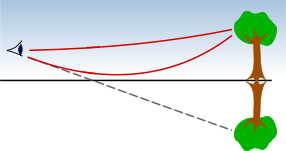
\includegraphics[width=12truecm]{slike/02_Fata1.jpg}
\caption{Zračno zrcaljenje na vročih tleh}
\label{fig:02_Fata1}
\end{figure}
\vglue-0.6truecm
Zgornje zračno zrcaljenje se nasprotno pojavi, 
kadar je spodnja plast zraka izrazito hladnejša od zgornjih plasti. 
Takrat se svetlobni žarki krivijo navzdol (slika~\ref{fig:02_Fata2})
in navidezno sliko predmeta premaknejo nad njegovo dejansko lego. 
Slika je lahko pokončna ali obrnjena, odvisno od oddaljenosti predmeta
in temperature plasti. 
\begin{figure}[h!]
\centering
\includegraphics[width=12truecm]{slike/02_Fata2.jpg}
\caption{Zračno zrcaljenje na hladnejši podlagi (Foto: Craig Clements, Wikimedia)}
\label{fig:02_Fata2}
\end{figure}
\vglue-0.6truecm
Ukrivljena pot žarkov zaradi temperaturnega gradienta v atmosferi
vodi še do enega zanimivega pojava: popačenja oblike Sonca ob sončnem 
zahodu. Ker žarki s spodnjega dela Sonca potujejo po bolj ukrivljeni
poti kot žarki z zgornjega dela, se spodnji rob navidezno premakne navzgor 
in slika Sonca se splošči ali popači.
\begin{figure}[ht]
\centering
\includegraphics[width=5truecm]{slike/02_Sonce.jpg}
\caption{Sonce se ob sončnem zahodu navidezno splošči in njegova oblika popači.}
\label{fig:02_Sonce}
\end{figure}
\vglue-0.6truecm
\section{Transformacije žarkov z matrikami ABCD}
V prejšnjem razdelku smo zapisali žarkovno enačbo v obosnem 
približku (enačba~\ref{eq:02_24}). Ključna parametra za opis trajektorije žarka sta 
oddaljenost od optične osi $z$, ki jo označimo z $x$, in naklonski 
kot žarka glede na optično os, ki ga označimo s $\vartheta$.
Naša naloga je povezati dve točki žarka na različnih mestih v
prostoru in zapisati preslikavo med njima, če je med točkama
optični medij oziroma nek optični element. 
\begin{figure}[ht]
\centering
\def\svgwidth{90truemm} 
\input{slike/02_ABCD0.pdf_tex}
\caption{Pri danem $z$ žarek opišemo z lego $x$ in smerjo $\vartheta$. Spremembo
teh dveh parametrov opišemo s preslikavo.}
\label{fig:01_ABCD0}
\end{figure}

V splošnem vrednosti lege in naklona v točki 2 izrazimo kot 
linearno kombinacijo prvotnih vrednosti v točki 1:
\begin{align}
 x_2 = & A x_1 + B \vartheta_1 \qquad \mathrm{in}  \label{eq:02_29}\\
 \vartheta_2 = & C x_1 + D\vartheta_1.
 \label{eq:02_30}
\end{align}
Če združimo parametra $x$ in $\vartheta$ v neki točki prostora
v dvodimenzionalni vektor,
lahko preslikavo strnjeno zapišemo v matrični obliki:
\boxeq{eq:02_31}{
\left[\begin{array}{c}
x_2\\
\vartheta_2
\end{array}\right] = 
\left[\begin{array}{cc}
A& B\\
C&D
\end{array}\right]
\left[\begin{array}{c}
x_1\\
\vartheta_1
\end{array}\right]
= M \left[\begin{array}{c}
x_1\\
\vartheta_1
\end{array}\right]\!\!.
}
Matriko $M$ imenujemo transformacijska oziroma prehodna matrika 
vmesnega optičnega medija ali optičnega elementa. 

\begin{example}
\label{ex:ML}
{\bf Matrika ABCD za premik v homogeni snovi s konstantnim lomnim količnikom.} 
Prvi primer naj bo homogena snov, v kateri je lomni količnik konstanten in enak $n$. 
V točki 1 pri $z_1$ naj bosta komponenti vektorja enaki $x_1$ in 
$\vartheta_1$. Poiščimo vrednosti komponent vektorja, 
če se premaknemo za $L$ vzdolž optične osi sistema do $z_2$ 
(slika~\ref{fig:01_ABCD1}). 
\begin{figure}[ht]
\centering
\def\svgwidth{70truemm} 
\input{slike/02_ABCD1.pdf_tex}
\caption{K izračunu matrike ABCD za premik v homogeni snovi}
\label{fig:01_ABCD1}
\end{figure}

Naklon žarka se pri premiku ne spremeni, zato ostane $\vartheta_2 = \vartheta_1$. Spremeni
pa se odmik od optične osi, saj žarek ne potuje vzporedno z osjo $z$. 
Vrednost $x_2$ zapišemo kot:
\begin{equation}
 x_2 = x_1 + (z_2-z_1)\vartheta_1 = x_1 + L\vartheta_1.
\label{eq:02_32}
\end{equation}
Potem zapišemo sistem enačb:
\begin{align}
 x_2 =& 1\cdot x_1 + L\cdot \vartheta_1 \qquad \mathrm{in} \label{eq:02_33}\\
 \vartheta_2 =& 0\cdot x_1 + 1\cdot \vartheta_1.
 \label{eq:02_34}
\end{align}
Iz zapisa razberemo koeficiente matrike $M$ za homogeno snov dolžine $L$:
\begin{equation}
 M = \left[\begin{array}{cc}
1& L\\
0&1
\end{array}\right]\!\!.
 \label{eq:02_35}
\end{equation}
\end{example}

\begin{example}
\label{ex:Mmeja}
{\bf Matrika ABCD za prehod skozi ravno mejo med dvema snovema.} Naj svetloba vpada na 
mejo dveh snovi z različnima lomnima količnikoma $n_1$ in $n_2$. Za izračun 
prehodne matrike izberemo dve točki na žarku: eno tik pred mejo in eno tik za njo. 
Lega žarka se ob tem ne spremeni in $x_2 = x_1$. 
Spremeni pa se naklon žarka. 
\begin{figure}[ht]
\centering
\def\svgwidth{70truemm} 
\input{slike/02_ABCD2.pdf_tex}
\caption{K izračunu matrike ABCD za prehod skozi ravno mejo med dvema snovema}
\label{fig:01_ABCD2}
\end{figure}

Za majhne naklone lahko lomni zakon
(enačba~\ref{eq:lomnizakon}) razvijemo in dobimo:
\begin{equation}
n_1 \vartheta_1 = n_2 \vartheta_2.
 \label{eq:02_36}
\end{equation}
Sistem enačb je potem:
\begin{align}
 x_2 =& 1\cdot x_1 + 0\cdot \vartheta_1 \qquad \mathrm{in} \label{eq:02_37}\\
 \vartheta_2 =& 0\cdot x_1 + \frac{n_1}{n_2}\cdot \vartheta_1.
 \label{eq:02_38}
\end{align}
Matrika $M$ za prehod skozi mejo med dvema snovema je:
\begin{equation}
 M = \left[\begin{array}{cc}
1& 0\\
0&\frac{n_1}{n_2}
\end{array}\right]\!\!.
\label{eq:02_39}
\end{equation}
\end{example}

\begin{example}
\label{ex:MUmeja}
{\bf Matrika ABCD za prehod skozi ukrivljeno mejo med dvema snovema.} V prejšnjem 
primeru je bila meja med snovema z lomnima količnikoma $n_1$ in $n_2$ ravna, zdaj pa 
poglejmo še matriko za prehod skozi ukrivljeno mejo. Krivinski radij mejne ploskve
naj bo $R$, pri čemer $R$ štejemo pozitivno, če je meja konveksna glede na smer
naraščajočega $z$ oziroma če je središče krožnice za mejo med snovema. V primeru, 
da je središče krožnice, ki določa mejo med snovema, pred mejo, je meja konkavna, 
krivinski radij mejne ploskve pa negativen. 

Za izračun matrike ponovno izberemo dve točki, prvo tik pred mejo in 
drugo tik za njo. To pomeni, da se oddaljenost od optične osi
pri prehodu ohranja in $x_1 = x_2$. 

Izračun naklona žarka po prehodu je malo bolj zapleten. Za zapis lomnega 
zakona moramo namreč vpeljati kote glede na normalo na
mejo. Vpadni kot je tako $\alpha = \vartheta_1 + \varphi$, lomni kot pa 
$\beta = \vartheta_2 + \varphi$ (glej sliko~\ref{fig:02_ABCD3}).
S slike razberemo, da velja zveza:
\begin{equation}
 \sin \varphi = \frac{x_1}{R} \approx \varphi,
 \label{eq:02_40}
\end{equation}
pri čemer smo privzeli, da so žarki blizu optične osi. 
\begin{figure}[!h]
\centering
\def\svgwidth{70truemm} 
\input{slike/02_ABCD3.pdf_tex}
\caption{K izračunu matrike ABCD za prehod skozi ukrivljeno mejo med dvema snovema}
\label{fig:02_ABCD3}
\end{figure}

Zapišemo lomni zakon,
pri čemer privzamemo, da so vsi koti majhni:
\begin{equation}
n_1 (\vartheta_1 + \varphi) = n_2 (\vartheta_2 + \varphi).
\label{eq:02_41}
\end{equation}
Od tod izračunamo kot $\vartheta_2$:
\begin{equation}
 \vartheta_2 = \frac{n_1-n_2}{n_2}\varphi + \frac{n_1}{n_2} \vartheta_1.
 \label{eq:02_42}
 \end{equation}
Če $\varphi$ izrazimo iz enačbe~(\ref{eq:02_40}), zapišemo transformacijo koordinat:
\begin{align}
 x_2 =& 1\cdot x_1 + 0\cdot \vartheta_1 \qquad \mathrm{in} \\
 \vartheta_2 =& \frac{n_1-n_2}{n_2R}\cdot x_1 + \frac{n_1}{n_2}\cdot \vartheta_1.
 \label{eq:02_43}
\end{align}
Razberemo matriko $M$ za prehod skozi ukrivljeno mejo med dvema snovema:
\begin{equation}
M = \left[\begin{array}{cc}
1& 0\\
\frac{n_1-n_2}{n_2R}&\frac{n_1}{n_2}
\end{array}\right]\!\!.
 \label{eq:02_44}
\end{equation}
V limitnem primeru, ko gre $R \to \infty$, se matrika prevede na matriko za
prehod skozi ravno mejo (glej primer~\ref{ex:Mmeja}).
\end{example}

Izračunajmo še determinanto izpeljanih matrik ABCD. Na splošno velja, da
je determinanta matrike ABCD enaka razmerju lomnih količnikov začetne in 
končne snovi. Če je lomni količnik snovi na koncu enak
kot na začetku (primer~\ref{ex:ML}), je $\det(M) = 1$, v nasprotnem primeru 
(primera~\ref{ex:Mmeja} in \ref{ex:MUmeja}) je $\det(M) = n_1/n_2$.

Do zdaj smo obravnavali matrike za posamezne prehode. Poglejmo, kako izračunamo
prehodno matriko za primer, če svetloba potuje skozi več elementov zapored. V tem
primeru se pokažeta izjemna praktičnost in uporabnost zapisa z matrikami, saj ob prehodu svetlobe skozi 
več elementov matrike za te elemente preprosto zmnožimo. Paziti moramo seveda
na vrsti red: matriko za element, na katerega vpade svetloba najprej, zapišemo
najbolj desno, to je najbliže vektorju, ki opisuje vpadno svetlobo. Celoten prehod
spet opiše ena sama matrika:
\begin{equation}
\left[\begin{array}{c}
x_N\\
\vartheta_N
\end{array}\right] 
= \tilde{M} \left[\begin{array}{c}
x_1\\
\vartheta_1
\end{array}\right]\!\!,
 \label{eq:02_45}
\end{equation}
pri čemer je:
\begin{equation}
\tilde{M} = M_N \cdot M_{N-1}~...~M_2 \cdot M_1.
 \label{eq:02_46}
\end{equation}
\begin{figure}[ht]
\centering
\def\svgwidth{100truemm} 
\input{slike/02_MMM.pdf_tex}
\caption{Prehod žarka skozi več optičnih elementov zapišemo kot produkt matrik posameznih prehodov.
Pri tem moramo paziti na vrstni red zapisa matrik.}
\label{fig:01_MMM}
\end{figure}

\section{Leče in zrcala}
Uporabimo matrike ABCD za izračun prehoda svetlobe skozi tanko lečo. Matriko
za prehod skozi lečo zapišemo kot produkt dveh matrik: prve, ki opiše
prehod skozi prvo ukrivljeno ploskev s krivinskim polmerom $R_1$, 
in druge, ki opiše prehod skozi izhodno ukrivljeno ploskev s 
krivinskim radijem $R_2$. Oglejmo si primer bikonveksne leče,
za katero je krivinski radij prve ploskve pozitiven, druge pa negativen
(slika~\ref{fig:02_tankaleca}). Lomni količnik leče naj bo $n_2$ in 
snovi okoli leče (navadno je to zrak) $n_1$.
\begin{figure}[!h]
\centering
\def\svgwidth{70truemm} 
%\input{slike/02_tankaleca.pdf_tex}
\caption{K izračunu matrike ABCD za prehod skozi tanko bikonvkesno lečo}
\label{fig:02_tankaleca}
\end{figure}

Ker smo privzeli, da je leča tanka, vmesne matrike za premik po prostoru 
ne zapišemo. Dobimo:
\beq
 M = \left[\begin{array}{cc}
1& 0\\
\frac{n_2-n_1}{n_1R_2}&\frac{n_2}{n_1}
\end{array}\right]\cdot 
\left[\begin{array}{cc}
1& 0\\
\frac{n_1-n_2}{n_2R_1}&\frac{n_1}{n_2}
\end{array}\right] = 
\left[\begin{array}{cc}
1& 0\\
\frac{n_2-n_1}{n_1}\left(\frac{1}{R_2}-\frac{1}{R_1}\right)&1
\end{array}\right]\!\!.
\label{eq:02_47}
\eeq
Vpeljimo nov parameter $f$, za katerega velja:
\beq
\frac{1}{f} = \frac{n_2-n_1}{n_1}\left(\frac{1}{R_1}-\frac{1}{R_2}\right)\!\!,
\label{eq:02_48}
\eeq
tako da spodnji levi element matrike zapišemo kot $-1/f$. Pomen tega parametra
bomo spoznali v nadaljevanju.

Uporabimo zdaj matriko za izračun prehoda svetlobe skozi lečo. Naj žarek izhaja iz 
predmeta, ki je na oddaljenosti $a$ od leče, opazujemo pa ga na razdalji
$b$ za lečo. Za prehod žarka moramo zmnožiti tri matrike: matriko za 
premik do leče, matriko za prehod skozi lečo in matriko za premik do opazovalca.
Dobimo:
\beq
M = 
\left[\begin{array}{cc}
1& b\\
0&1
\end{array}\right]\cdot
\left[\begin{array}{cc}
1& 0\\
-\frac{1}{f}&1
\end{array}\right]
\cdot
\left[\begin{array}{cc}
1& a\\
0&1
\end{array}\right]
= 
\left[\begin{array}{cc}
1-\frac{b}{f}& a+b-\frac{ab}{f}\\
-\frac{1}{f}&1-\frac{a}{f}
\end{array}\right]\!\!.
\label{eq:02_49}
\eeq

Če želimo, da na desni strani leče nastane prava slika predmeta, se morajo vsi
žarki, ki izhajajo iz ene točke predmeta (neodvisno od njihovega naklona), zbrati
v eni točki. Ta zahteva je izpolnjena le ob pogoju, da je element $B = 0$
in velja:
\boxeq{eq:PreslikavaLeca}{
\frac{1}{f} = \frac{1}{a}+\frac{1}{b}.
}
Dobili smo enačbo leče.

Razmerje med velikostjo slike $x_2$ in velikostjo predmeta $x_1$ določa
element matrike $A$, ki ga z upoštevanjem enačbe~(\ref{eq:PreslikavaLeca})
zapišemo kot:
\beq
A= 1-\frac{b}{f} = 1 - b\left(\frac{1}{a}+\frac{1}{b}\right) = -\frac{b}{a}.
\label{eq:02_50}
\eeq
Povečava leče je tako:
\boxeq{eq:PovecavaLece}{
\frac{x_2}{x_1} =-\frac{b}{a},
}
pri čemer negativni predznak pomeni obrnjeno sliko 
(glej sliko~\ref{fig:02_slikazaleco}).
\begin{figure}[!h]
\centering
\def\svgwidth{70truemm} 
%\input{slike/02_slikazaleco.pdf_tex}
\caption{Nastanek prave (levo) in navidezne (desno) slike pri prehodu
skozi tanko bikonveksno lečo}
\label{fig:02_slikazaleco}
\end{figure}

Če je $a<f$, je po enačbi~(\ref{eq:PreslikavaLeca}) vrednost $b$ negativna. 
Žarki desno od leče se ne sekajo, temveč se sekajo podaljški 
žarkov levo od leče. Slika predmeta je tako le navidezna in je
ne moremo projicirati na zaslon. Povečava take slike je pozitivna, 
kar pomeni, da je navidezna slika pravilno obrnjena. 

Za konec poglejmo še pomen parametra $f$, ki smo ga vpeljali z enačbo~(\ref{eq:02_48}).
Poglejmo, v kaj se preslika žarek, ki na poljubni oddaljenosti od osi $x$ vpada na lečo 
vzporedno z optično osjo $z$:
\beq
\left[\begin{array}{c}
x_2\\
\vartheta_2
\end{array}\right] =
\left[\begin{array}{cc}
1-\frac{b}{f}& a+b-\frac{ab}{f}\\
-\frac{1}{f}&1-\frac{a}{f}
\end{array}\right] \cdot
\left[\begin{array}{c}
x\\
0
\end{array}\right] = 
\left[\begin{array}{c}
\left(1-\frac{b}{f}\right)x\\
-\frac{x}{f}
\end{array}\right]\!\!.
\label{eq:02_51}
\eeq
Da bo lega slike neodvisna od $x$ in se bodo vsi vzporedni žarki zbrali 
v eni točki, mora veljati $1-b/f = 0$ in $b=f$. Parameter $f$ torej 
prestavlja goriščno razdaljo leče. 

Ker navadno obravnavamo lečo v zraku, lahko poenostavljeno zapišemo goriščno
razdaljo leče kot:
\boxeq{eq:goriscna}{
\frac{1}{f} = \left(n-1\right)\left(\frac{1}{R_1}-\frac{1}{R_2}\right)\!\!,
}
pri čemer je $n$ lomni količnik stekla, iz katerega je leča narejena.

Opisani izračun je bil narejen na primeru bikonveksne leče, ampak velja
povsem splošno za poljubno tanko lečo. Paziti moramo le na predznake krivinskih
radijev vstopne in izstopne ploskve. Če je ena stranica leče ravna, je 
njen krivinski radij neskončen. 

\begin{example}{\bf Preslikava z dvema zaporednima lečama}
Poglejmo prehod svetlobe skozi dve zaporedni tanki leči z goriščnima
razdaljama $f_1$ in $f_2$, ki sta na medsebojni oddaljenosti $s$.
\begin{figure}[!h]
\centering
\def\svgwidth{70truemm} 
%\input{slike/02_lecje.pdf_tex}
\caption{Prehod svetlobe skozi sistem dveh tankih leč}
\label{fig:02_lecje}
\end{figure}

Matriko 
za prehod z leve proti desni zapišemo kot:
\beq
M = 
\left[\begin{array}{cc}
1& 0\\
-\frac{1}{f_2}&1
\end{array}\right]\cdot 
\left[\begin{array}{cc}
1& s\\
0&1
\end{array}\right]\cdot
\left[\begin{array}{cc}
1& 0\\
-\frac{1}{f_1}&1
\end{array}\right] = 
\left[\begin{array}{cc}
1-\frac{s}{f_1}& s\\
-\frac{1}{f_1}-\frac{1}{f_2}+\frac{s}{f_1f_2}&1-\frac{s}{f_2}
\end{array}\right]\!\!.
\label{eq:02_54}
\eeq
Izračunajmo zdaj goriščno razdaljo takega sistema in lego gorišča
na desni strani. Za opis  žarkov desno
od sistema je treba matriko prehoda pomnožiti še z matriko premika. 
Naj bodo vpadni žarki vzporedni z optično ravnino in jih zapišemo 
v obliki vektorja $(x_1,0)$. Izhodne žarke potem izračunamo kot:
\beq
\left[\begin{array}{c}
x_2\\
\vartheta_2
\end{array}\right]
 = 
\left[\begin{array}{cc}
1& d\\
0&1
\end{array}\right]
\cdot
\left[\begin{array}{cc}
A& B\\
C&D
\end{array}\right]\cdot 
\left[\begin{array}{c}
x_1\\
0
\end{array}\right] = 
\left[\begin{array}{c}
\left(A+dC\right)x_1\\
Cx_1
\end{array}\right]\!\!,
\label{eq:02_55}
\eeq
pri čemer so elementi matrike podani z enačbo~(\ref{eq:02_54}). 
Po definiciji se vzporedni vpadni žarki po prehodu sekajo v gorišču, 
zato je naklon izhodnega žarka $\vartheta_2 = -x_1/f$ in $C = -1/f$. 
Od tod razberemo goriščno razdaljo sistema:
\boxeq{eq:lecje}{
\frac{1}{f} = \frac{1}{f_1} + \frac{1}{f_2} - \frac{s}{f_1f_2}.
}
Oddaljenost gorišča od desne leče določimo iz pogoja, da je v gorišču $x_2 = 0$. Dobimo:
\beq
d = -\frac{A}{C} = \frac{f_1f_2-sf_2}{f_1+f_2-s}.
\label{eq:02_56}
\eeq

Pri sestavu leč vpeljemo še glavno ravnino, to je ravnino, v kateri bi 
bila postavljena nadomesta tanka leča. Dobimo jo tako, da poiščemo 
presečišče žarkov, ki vpadajo na sistem vzporedno z optično osjo, 
in žarkov, ki iz sestava izhajajo desno od lečja. Lego glavne ravnine je preprosto
določiti, saj vemo, da je gorišče od glavne ravnine oddaljeno ravno 
za goriščno razdaljo. Ker oba parametra poznamo, lahko hitro izračunamo
tudi lego glavne ravnine.

Račun, ki smo ga naredili do zdaj, je bil narejen za prehod svetlobe iz
leve proti desni strani. Ker se leči v splošnem razlikujeta in matrike
ne komutirajo, je prehod z desne proti levi drugačen. Skupna goriščna
razdalja ostane enaka, premakneta pa se lega gorišča (ki ga imenujemo
levo gorišče) in glavne ravnine.

Poglejmo za konec še pogoj, pri katerem so izhodni žarki iz sistema 
vzporedni z optično osjo. Da to velja pri vseh vstopnih $x$, mora biti 
element matrike $C$ enak nič in:
\beq
s = f_1 + f_2.
\label{eq:02_57}
\eeq
Povečava takega sistema je z upoštevanjem enačbe~(\ref{eq:02_57}) enaka:
\beq
\frac{x_2}{x_1} = 1 - \frac{s}{f_1} = \frac{f_2}{f_1}.
\label{eq:02_58}
\eeq
Postavitev dveh leč na oddaljenost, ki je enaka vsoti goriščnih razdalj
leč, je praktično zelo pomembna, saj predstavlja postavitev leč pri 
daljnogledu oziroma teleskopu.
\end{example}

\begin{example}{\bf Preslikava z debelo lečo}
Matriko za prehod skozi debelo lečo s krivinskima radijema
$R_1$ in $R_2$ ter debelino $d$ lahko neposredno izračunamo
z množenjem treh matrik: matrike za prehod skozi ukrivljeno vstopno 
ploskev, matrike za premik in matrike za prehod skozi ukrivljeno izstopno ploskev:
\beq
M = 
\left[\begin{array}{cc}
1& 0\\
\frac{n-1}{R_2}&n
\end{array}\right]
\cdot
\left[\begin{array}{cc}
1& d\\
0&1
\end{array}\right]
\cdot
\left[\begin{array}{cc}
1& 0\\
\frac{1-n}{nR_1}&\frac{1}{n}
\end{array}\right]
\label{eq:02_52}
\eeq
Pri tem smo privzeli, da je leča v zraku in $n_1 = 1$.

Matriko za prehod pa lahko izračunamo še na podlagi podobnosti 
s sistemom dveh leč. Razdelimo debelo lečo
na tri dele: vstopno plankonveksno lečo, plast stekla in izstopno plankonkavno lečo.
Goriščni razdalji leč potem zapišemo kot (enačba~\ref{eq:goriscna}):
\beq
\frac{1}{f_1} = (n-1)\frac{1}{R_1}\qquad \mathrm{in} \qquad \frac{1}{f_2} = (n-1)\frac{-1}{R_2}.
\label{eq:02_53}
\eeq
Pri vmesnemu prehodu skozi plast stekla moramo upoštevati njegov
lomni količnik. Na splošno se pri prehodu žarka skozi plast snovi debeline $d$
z lomnim količnikom $n$ matrika zapiše kot:
\beq
M = 
\left[\begin{array}{cc}
1& 0\\
0&n
\end{array}\right]\cdot
\left[\begin{array}{cc}
1& d\\
0&1
\end{array}\right]\cdot
\left[\begin{array}{cc}
1& 0\\
0&\frac{1}{n}
\end{array}\right] = 
\left[\begin{array}{cc}
1& \frac{d}{n}\\
0&1
\end{array}\right]\!\!.
\label{eq:02_54}
\eeq
Vidimo, da se efektivna dolžina poti skrajša za faktor $n$.

Ugotovitve vstavimo v enačbo za lečje (enačba~\ref{eq:02_54}) in dobimo:
\beq
M = 
\left[\begin{array}{cc}
1-\frac{d}{nf_1}& \frac{d}{n}\\
-\frac{1}{f_2}-\frac{1}{f_1}+\frac{d}{nf_1f_2}&1-\frac{d}{nf_2}
\end{array}\right]\!\!.
\label{eq:02_53}
\eeq
Hitro lahko preverimo, da dobimo isti rezultat, če zmnožimo matrike v enačbi~(\ref{eq:02_52}).
Prav tako hitro preverimo tudi, da je izračunana matrika za debelo lečo v limitnem 
primeru $d \to 0$ enaka matriki za prehod skozi tanko lečo. 
\end{example}
 
\subsection*{Odboj svetlobe na zrcalih}
Obravnavajmo na kratko še odboj svetlobe na zrcalih. Pri ravnih zrcalih je 
preprosto. Vse slike posamezne točke se po odboju zberejo v eni točki, navidezna slika, 
ki pri tem nastane, pa je enako velika in enako obrnjena kot predmet.

Bolj zanimiva je obravnava krogelnih zrcal. Tudi 


\section{Optične naprave}

mikroskop, daljnogled, spektroskop, oko, korekcijska očala. Kaj astronomskega? Nujno dodati.


